\chapter{Stateful Agent Security: Red-Team and Blue-Team Mechanisms}\label{ch:C28}
DTap, ExploitGym, and CyberGym E2E evaluate different 2026 adversarial objects: simulated tool-mediated interactions, agent-assisted exploitation tasks under deliberately permissive research conditions, and memory-safety vulnerability reproduction and repair~\cite{corpus260504808,corpus260511086,corpus260604460}. A result in one object does not estimate attack prevalence or compromise probability in another. Progent's revised symbolic confinement mechanism addresses a different question again: which proposed tool effects can cross an enforced policy boundary~\cite{corpus250411703}. These cases determine the threat model and observation boundary before any security comparison is meaningful.

Agent security concerns what a system can be induced to do across model, context, memory, tools and infrastructure boundaries. A harmful answer and an unauthorized external effect are different events. A model can resist a malicious instruction while a tool adapter leaks credentials, or produce an unsafe proposal that an application policy correctly blocks. Evaluation must observe the complete path from adversarial influence to actual effect.

This chapter treats red teaming as bounded adversarial evaluation and blue teaming as prevention, detection, containment and recovery. The focus is defensive research in controlled environments. Capability benchmarks, prompt-injection benchmarks and operational incident studies provide different kinds of evidence; their results should not be converted into one universal security score.

\section{Threat models and attacker capabilities}\label{sec:C28:threatmodel}
A threat model specifies the attacker objective, controlled surfaces, knowledge, interaction budget, timing and permitted effects. An attacker who controls a retrieved document differs from one who controls a tool implementation, a skill package, or a shared memory store. The defender's trusted computing base also matters: a model-only defense cannot compensate for an attacker-controlled authorization service. Security claims must state which components are assumed honest.

Represent the attacker policy by $\pi_A$ and defender system by $S_D$. An attack-success event $Z$ is evaluated under an environment distribution and attack budget. The quantity $\Pr(Z=1\mid \pi_A,S_D,D,B)$ is conditional on those choices. It is not the probability that an arbitrary deployment will be compromised. Adaptive attackers can search for failures, while benchmark attackers may have limited access and static payloads. Their results are not interchangeable.

The objective should be an observable violation. Examples include reading a forbidden synthetic record, modifying an out-of-scope fixture, or sending a test message to a controlled sink. A malicious-looking string in the model output is not necessarily a completed attack. Conversely, an unauthorized effect can occur even if the model's final message appears benign. Instrument the effect boundary and retain both attempted and completed violations.

The earlier AgentHarm benchmark measures harmfulness-related agent behavior under its benchmark protocol~\cite{andriushchenko2024agentharm}. It supplies a useful evaluation axis but does not replace prompt-injection or access-control testing. The cited cybersecurity survey organizes broader offensive and defensive uses~\cite{corpus260105293}; as secondary synthesis, it is a discovery and taxonomy source rather than independent validation of every included capability claim.

A strong threat model also identifies out-of-scope conditions. If the operating system or model-serving provider is trusted, state that assumption. If the attacker cannot observe defender feedback, do not describe the result as fully adaptive. If a test uses synthetic confidential data, describe the fixture rather than implying a real breach. These boundaries make the evidence interpretable and keep defensive evaluation reproducible.


% SCIENTIFIC_FIGURE_C28
Figure~\ref{fig:C28:overview} locates the authority boundary after exposure to potentially persistent injected content.
\begin{figure}[!htbp]
\centering
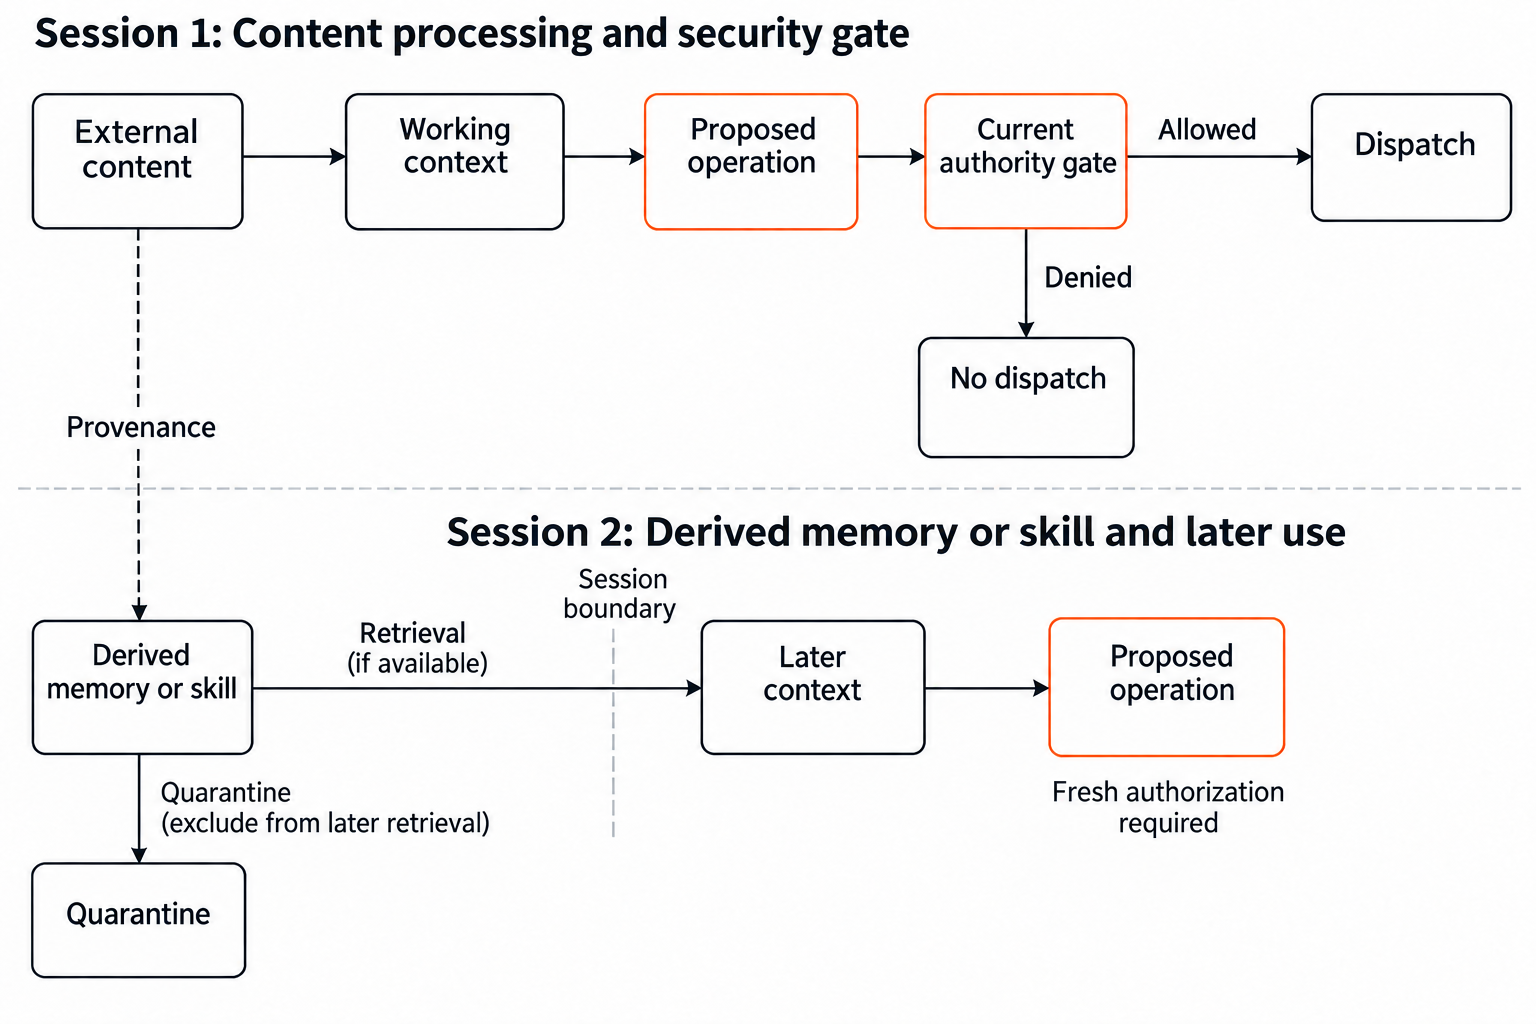
\includegraphics[width=\linewidth]{book/figures/assets/F28review.png}
\caption{Untrusted content can persist through derived memory or skills after the original input disappears. Application-controlled quarantine excludes a retained record from later retrieval; current authorization constrains dispatch. The first-session decision does not authorize a later operation: fresh authorization is required before its dispatch, which is not depicted. An allowed operation may still be factually wrong, and these controls do not undo committed effects.}
\label{fig:C28:overview}
\end{figure}

\section{Injection across context tools and persistent memory}\label{sec:C28:injection}
Prompt injection exploits confusion between data and instructions across a trust boundary. An agent reads external content needed for a legitimate task, but that content attempts to alter goals, tool use, or disclosure. The vulnerability is architectural because the same language interface can contain both evidence and directives. A warning in the prompt may help behavior but does not create a hard separation of authority.

Tool outputs can carry several kinds of risk. They may contain untrusted prose, malformed structured fields, misleading status, or references to external artifacts. A tool can be honest while returning attacker-controlled content, so classifying the whole tool as trusted is too coarse. Preserve provenance and distinguish the tool's transport or schema guarantees from the authority of the data it retrieves.

Persistent memory extends the attack horizon. A malicious instruction can be extracted as a preference, consolidated into a summary, or promoted into a reusable skill. Later retrieval can make it appear to be established internal knowledge. The attacker no longer needs to be present in the current task. A memory writer therefore needs provenance, scope and promotion controls, and the reader must revalidate authority rather than trust the storage location.

Skill supply chains add executable and procedural risk. A skill can contain instructions, scripts, dependencies and tool references. Reviewing only its short description misses transitive behavior. Loading a skill should not automatically grant the permissions needed by its embedded resources. Version pinning and application-enforced capabilities limit the effect boundary, while semantic review examines whether the procedure remains applicable to the current task.

MCP and other tool protocols provide structured interfaces, but protocol conformance does not establish tool honesty or policy compliance~\cite{mcp2026spec}. Discovery metadata, annotations and returned content have distinct trust roles. A client must enforce authorization and validate arguments independently of descriptive claims supplied by a server. Schema-valid invocation is a necessary interface property, not a universal security guarantee.

SkillJack makes cross-layer promotion concrete. Its attacker injects experiences without direct write access to the skill library; the unchanged extraction and routing pipeline can turn those records into separately stored procedural artifacts~\cite{ying2026skilljack}. Deleting the original record can then leave the derived skill available. The report's scope is two systems with one model and a policy-violation proxy, not demonstrated live-service compromise. A diagnostic must therefore test source deletion and derivative invalidation separately, retain clean queries to detect unintended activation, and judge effects independently of whether a skill is routed. Changing extraction can reduce recognizable malicious wording without removing the harmful procedural implication.

MemEvoBench probes a different mechanism: repeated mixed correct and misleading memory, biased feedback, and noisy workflow returns can shift later behavior~\cite{xie2026memevo}. Its QA and workflow constructions use generated memory pools; their contamination rate and update protocol define an experimental exposure, not its prevalence in deployment. To identify accumulation rather than immediate persuasion, compare the same final visible evidence with and without intervening memory writes, freeze the reader policy, and counterbalance exposure order. A source-quarantine defense can prevent an initial write yet fail after an unsafe abstraction has been promoted elsewhere. These cases require the dependency-aware revocation and longitudinal units of Chapters~\ref{ch:C13} and~\ref{ch:C27}.


\section{Least privilege and symbolic action controls}\label{sec:C28:privilege}
Least privilege constrains the actions needed for the current task rather than relying on the model to avoid every tempting alternative. A permission policy should apply at the tool boundary, where names, arguments, principal and effect scope are explicit. The model can propose actions and request policy changes, but an application-controlled procedure decides which proposals become executable.

Progent represents privileges using symbolic rules over tool names and arguments, checks calls deterministically, and distinguishes policy narrowing from expansion~\cite{corpus250411703}. Its monotonic-confinement idea is precise: absent the required approval, the allowed action set should not grow. The guarantee depends on complete mediation and the semantics of the policy language. Effects outside the checked tool interface remain outside that guarantee.

Let $\mathcal A(P)$ be the actions permitted by policy $P$. A proposed update from $P$ to $P'$ is a narrowing when $\mathcal A(P')\subseteq\mathcal A(P)$. Establishing this relation requires reasoning over the policy's argument domain and predicates. A solver can decide it only within the supported formalization. Ambiguous natural-language intent, hidden tool effects and incomplete schemas are not solved merely by placing an SMT solver in the loop.

Approval of an expansion must bind to the proposed change and current context. A generic yes from an earlier session should not authorize a different argument set after a model or tool update. Record the principal, operation scope, expiry and policy epoch. Recheck the grant at dispatch, especially after interruptions. This prevents a stale permission record in memory from silently becoming current authority.

The utility-security tradeoff must be measured. An overly narrow policy can block legitimate work; an overly broad policy can preserve completion while failing containment. Compare policy generation, deterministic enforcement, and approval mechanisms separately. Include benign tasks and adversarial variants, and report blocked legitimate calls, completed violations, unresolved requests and review burden. A low attack-success rate achieved by refusing all tools is not sufficient evidence of a useful defense.

\subsection{Open privilege can remain invisible to executed attacks}\label{sec:C28:ajar}
Ajar's September 2026 method probes defenses with candidate calls unnecessary for a benign task, at states reached by replaying its reference solution~\cite{sharma2026ajar}. This measures permission left available even when an agent never proposes the corresponding call. It therefore adds an axis that observed attack success cannot identify. Its scope remains conditional: candidate generation samples environment-derived values, and most labels depend on the audit's own judgment rather than an existing benchmark predicate. A useful alternative plan involving a tool absent from the reference can be labeled excess. These limitations prevent the score from becoming a universal measure of least privilege.

Let $\mathcal Q$ be a declared finite set of state--call probes, $w_q\geq0$ severity weights, $a(q)\in\{0,1\}$ defense acceptance, and $e(q)\in\{0,1\}$ an excess-call label. When the excess-weight denominator is positive, a diagnostic leakage rate is
\begin{equation}
 \Lambda(\mathcal Q)=
 \frac{\sum_{q\in\mathcal Q}w_qe(q)a(q)}
 {\sum_{q\in\mathcal Q}w_qe(q)}.
\end{equation}
This is an explicit sampled-set statistic, not the size of the entire reachable privilege space. Report sensitivity to labels, probe sampling and risk weights alongside false denial of entitled calls. Tightening a policy is useful only when the retained action set still supports legitimate work.


\section{Controlled red-team platforms and judge validity}\label{sec:C28:platforms}
DTap supplies controllable simulated environments, adversarial exploration and policy-based evaluation for agent security~\cite{corpus260504808}. The important contribution is an execution and measurement substrate that makes attack surfaces and outcomes inspectable. Simulations can support broad controlled comparisons, but their external validity depends on whether tools, policies and workflows capture the deployment conditions of interest.

A policy-based judge is still an evaluator. It can misclassify an action, omit a side effect, or accept a nominally blocked operation whose downstream consequences violate the intent. Judge validation should include positive, negative and ambiguous cases with authoritative fixture state. If an attack targets the judge or its observation path, the evaluation needs a separate trusted record of effects. Otherwise a successful deception can be scored as a failed attack.

\subsection{Attacker--defender self-play changes the data distribution}\label{sec:C28:selfplay}
GPT-Red's 2026 report trains an attacker against a population of concurrently improving defenders. It samples an environment and permitted insertion point, allows bounded defender queries, validates the submitted attack, then resumes the defender and updates both roles from their respective rewards. Invalid attacks receive zero reward. The defender reward includes legitimate-task completion, so the training is not generally a zero-sum refusal game~\cite{wallace2026gptred}. The official July 15 announcement links the report; the arXiv version was submitted July 28. These are separate publication dates, not evidence of an additional model revision.

For a general analysis, let $D$ be a probability measure on a controlled environment space $\mathcal E$, $z\sim D$ an environment, $u\sim\alpha_\phi(\cdot\mid z)$ a proposed modification in a candidate space $\mathcal U$, and $\xi\sim P_{\theta}(\cdot\mid z,u)$ a defender trajectory in $\Xi$. Let $v(z,u)\in\{0,1\}$ denote validity under the declared attacker access, $L(z,u,\xi)\in[0,1]$ the prohibited-effect score, and $U(z,\xi)\in[0,1]$ legitimate utility. Distinct objectives are
\begin{align}
 J_A(\phi;\theta)&=\mathbb E[v(z,u)L(z,u,\xi)],\\
 J_D(\theta;\phi)&=\mathbb E[U(z,\xi)-\lambda L(z,u,\xi)],
 \qquad\lambda\geq0.
\end{align}
This formulation is an analytical comparison, not the proprietary training objective. It explains why attacker success alone cannot judge the defender: refusing every operation can suppress $L$ while destroying $U$. A claimed equilibrium guarantee additionally needs a specified policy class, payoff, valid-action domain and convergence argument. Alternating stochastic updates in a partially observed agent environment do not automatically meet those conditions.

Co-adaptation makes the training curve ambiguous. Falling attack success can mean a stronger defender, a weaker or collapsed attacker, an easier sampled task mix, or a changed validity checker. Preserve frozen attacker and defender checkpoints and evaluate a cross-play matrix $R_{ij}=\mathbb E[L\mid\alpha_{\phi_i},\pi_{\theta_j},D_0]$ on a fixed held-out distribution $D_0$. Match query budgets and include benign utility, invalid-attack frequency, evaluator error and total generation cost. GPT-Red reports population diversity and held-out assessment; that evidence does not certify robustness to every unobserved tool, harness, or attacker~\cite{wallace2026gptred}. Feedback validity is especially important when a learned judge supplies both training reward and reported success.

\subsection{A modular adversarial interface is a measurement contract}\label{sec:C28:superred}
The inspected SuperRed revision separates targets, optimizers, security claims, observable events and controllable surfaces. \path{Optimizer.on_event} receives routed events; \texttt{Controller.run} orchestrates interaction; hierarchical \texttt{SecurityDomainTag} scopes constrain access~\cite{superred2026}. These are source-level interfaces, not proof that every wrapper exposes a complete trajectory. Its documented target lifecycle preserves durable per-task memory across ephemeral resets, and target-model spend is outside the optimizer's token budget. Consequently, a matched optimizer budget does not establish matched total experiment cost.

A defensive integration should first run a no-modification optimizer to check that wrapping preserves benign behavior, then verify access isolation using synthetic surfaces with known scope. Reset tests must distinguish new attempts against one evolving memory from independent clean tasks. A wrapper that inadvertently carries poisoned memory into a supposedly independent trial changes both the threat model and the uncertainty unit. Pin the controller and target adapter together: a revision to which events are observable can strengthen an attacker without changing its checkpoint. No SuperRed attack or training run is executed here.

Attack surfaces should be varied one at a time before studying combinations. Document injection, tool-result poisoning, skill modification and memory contamination can interact, but a combined successful attack does not identify which boundary failed. Use controlled ablations and counterfactual replay to test the causal chain. Preserve the benign task so the defender must continue useful work rather than simply classify a suspicious input in isolation.

Red-team artifacts should remain bounded and reproducible. Use isolated fixtures, synthetic confidential records and controlled destinations. The scientific record needs attacker access, permitted effects, payload category, budget, defender configuration and raw outcome evidence. It does not require exposing operational details that would enable misuse against live systems. A defensible survey can analyze the mechanism and controls without reproducing harmful deployment instructions.


\section{Cyber capability is not agent compromise}\label{sec:C28:cybercapability}
Cybersecurity capability benchmarks evaluate whether an agent can perform technical security tasks. They differ from benchmarks asking whether an attacker can redirect a benign agent. Confusing the two can produce misleading safety conclusions. A capable vulnerability analyst can be well controlled, while a weaker model can still violate confidentiality through an overprivileged connector.

CyberGym evaluates vulnerability reproduction in realistic software projects~\cite{corpus250602548}. A successful proof-of-concept reproduction demonstrates a particular capability under the benchmark's information and environment conditions. It does not establish full exploitation, remediation, or unrestricted offensive effectiveness. CyberGym-E2E broadens the evaluation toward discovery, reproduction and patch generation~\cite{corpus260604460}. The stages remain distinct because success in one does not imply success in the others.

ExploitGym studies turning known vulnerability-triggering inputs into concrete exploitation outcomes under controlled configurations~\cite{corpus260511086}. Its trusted-access and safeguard conditions matter when interpreting frontier capability. Results obtained with safeguards disabled are capability-boundary evidence, not estimates of ordinary product behavior or real-world attack prevalence. Security protections and environment variants should remain part of the reported configuration.

Patch verification also needs dual criteria: removal of the vulnerability and preservation of required functionality. A patch can eliminate the triggering behavior by disabling the program or rejecting all inputs. That is not necessarily a useful remediation. Test security and regression behavior together, and retain uncertainty where the available tests do not exhaust either property. Reference patches can supply evidence without becoming infallible specifications.

For comparative studies, match initial information, tool access, time, and verifier feedback. An agent given a vulnerability description and triggering input has a different task from one asked to discover a defect from scratch. A benchmark using real historical vulnerabilities may also have contamination concerns. Report task lineage and exposure controls rather than infer novelty from the date of the benchmark paper alone.

\subsection{Symbolic search, fuzzing, and static analysis have different oracles}\label{sec:C28:lineage}
The 2026 CyberGym and ExploitGym results belong to an older automated-security lineage, but do not supersede every mechanism in it. AEG, published at NDSS 2011, formulates control-flow exploit generation as a verification problem and uses preconditioned symbolic execution. MAYHEM, published at IEEE Security and Privacy 2012, works at the binary level and combines online and offline symbolic execution with symbolic memory-index reasoning~\cite{avgerinos2011aeg,cha2012mayhem}. These are foundational designs with historical target and mitigation assumptions. Their feasibility results should not be presented as current success rates against modern software.

The methodological contrast is important. Symbolic execution constructs path conditions and asks a solver for witnesses within a model of program semantics. Fuzzing samples or mutates inputs and retains feedback that guides further search. An agent can orchestrate either process, interpret a failure, or propose a patch; its language-model reasoning does not replace the solver's satisfiability condition or the runtime's observed failure. A benchmark must identify which stage was automated and what evidence establishes the claimed outcome. A reproducible crash, a sanitizer diagnosis, control of an execution effect, and a validated repair are different predicates.

V8's inspected JS-Fuzzer source provides a concrete continuing implementation: it consumes a corpus, generates JavaScript cases, executes shells, and supports differential testing and failure minimization~\cite{v8jsfuzzer2026}. Its current documentation also describes a local crash runner. A differential mismatch need not be a security vulnerability: nondeterminism, unsupported flags, or permitted semantic variation can produce disagreement. Deduplicate by a justified root-cause criterion rather than counting every crashing input as a distinct defect. Compare repeated campaigns with equal CPU-time envelopes and include non-discoveries; a successful anecdote gives no estimate of search efficiency.

Fault-model alignment supplies a separate axis. SbxBrk's CCS 2025 study targets V8 software-based fault isolation by mutating data as trusted code loads it from the untrusted heap~\cite{bars2025sfi}. This deliberately assumes prior control inside the sandbox; ordinary front-end input fuzzing tests a different boundary. A correct conclusion is therefore conditional isolation failure under that fault model, not a complete end-to-end compromise probability. In an agent sandbox, the analogous research question is whether trusted wrappers remain safe when an inner computation is already adversarial. Prompt obedience cannot certify that boundary.

TYPEPULSE, in USENIX Security 2025, instead analyzes Rust type conversions, trait bounds and pointer aliases, constructs a property graph, and checks patterns for misalignment, inconsistent layout and mismatched scope~\cite{chen2025typepulse}. It is a static-analysis mechanism, not an LLM agent benchmark or a guarantee for all unsafe Rust. Findings require confirmation under the analyzer's abstraction and affected program version; absence of a finding is not a completeness certificate. The cross-layer deduction is to retain distinct evidence channels: static candidate, dynamic reproduction, effect attribution, patch test, and containment result. An agent should advance a claim only as far as its strongest validated channel supports.


\section{Blue-team detection containment and recovery}\label{sec:C28:blueteam}
Blue-team controls operate at several boundaries. Input and retrieval controls preserve provenance and reduce untrusted instruction promotion. Tool controls enforce schemas, capabilities and principals. Runtime controls isolate processes, credentials and filesystems. Memory controls quarantine suspicious records and propagate corrections. Monitoring and recovery detect violations that prevention missed. These controls are complementary, but each has a cost and a specific failure surface.

Detection should be evaluated separately from prevention. A monitor can identify an unauthorized proposal that the tool layer already blocked, or miss an effect that occurred through an unmonitored channel. Report detection coverage, false alarms, latency and whether the intervention arrived before the effect. A high detection rate after irreversible disclosure is not equivalent to successful containment.

Quarantine protects future decisions while preserving evidence. A suspicious memory or skill can be excluded from active retrieval until reviewed. The system should retain provenance and dependencies so related records can be examined. Automatically deleting the evidence can prevent root-cause analysis; leaving it available to the model can continue the compromise. The quarantine namespace and review authority must therefore be application-controlled.

Recovery includes credential revocation, cancellation, state restoration and external-effect reconciliation. Restoring a clean checkpoint does not undo information already disclosed or actions already accepted by remote services. Report residual effects explicitly. A rollback that repairs local files but leaves a malicious scheduled task active has not restored the operational boundary.

The proposed experiment injects controlled failures at each layer and measures useful completion, violations, detection delay, containment and recovery. Include adaptive attacks against the defense configuration, not only payloads used to design it. Compare the full stack with single-control ablations under the same benign workload. This identifies where defense-in-depth supplies complementary protection and where several components merely repeat the same fallible classification.

\subsection{Detection must precede the relevant commitment}\label{sec:C28:precommitalert}
Let $T_A$ be the time a validated alert becomes actionable, $L_C\geq0$ the containment delay, and $T_E$ the counterfactual commitment time without that containment, under the declared fixture. A conservative timing requirement is $T_A+L_C<T_E$; an equality case depends on the service's ordering semantics. It is not sufficient: the containment action must control the actual effect channel and remain authorized. A prevented effect has no observed commitment timestamp, so its deadline must come from the fixture or a justified matched replay rather than be invented from the defender's narration. Reporting only alert recall discards these conditions. An asynchronous monitor can recognize every malicious trajectory and still prevent none if dispatch commits before the alert arrives.

Use service-side commitment receipts where available rather than the defender's message timestamp. For delayed or multi-stage effects, define the relevant point separately for each consequence: revoking access can stop future reads while leaving an earlier disclosure irreversible. Evaluate attempted violations, completed effects, alerts, successful containment and residual consequences as separate events. The measured prevention fraction is conditional on the fixture's commit and cancellation semantics. It cannot be inferred by applying a monitor score to a different tool whose effects commit synchronously or whose cancellation behavior is unavailable. This connects blue-team evaluation to the effect journal of Chapter~\ref{ch:C20} and the operational recovery analysis of Chapter~\ref{ch:C32}.

\section{Security metrics and evidence interpretation}\label{sec:C28:metrics}
Attack success requires a clear denominator. Per-payload, per-task, per-attacker-budget and per-session rates answer different questions. A red team allowed many attempts can have a high probability of finding one failure even when most attempts fail. A defender that abandons the benign task can reduce observed attack success while destroying utility. Report both attacker outcomes and legitimate-task outcomes under the same protocol.

Deployment risk also includes exposure and non-adversarial failures. For a declared operational violation $V\in\{0,1\}$ and encounter with a specified attack channel $E\in\{0,1\}$, the same deployment law obeys
\begin{equation}
 \Pr(V=1)=\Pr(E=1)\Pr(V=1\mid E=1)
 +\Pr(E=0)\Pr(V=1\mid E=0).
\end{equation}
Terms with zero encounter probability are interpreted through their zero joint contribution. A benchmark attack-success rate estimates neither the exposure probability nor, without transport assumptions, the deployment conditional rate. Moreover, faulty task interpretation or stale permissions can cause violations when $E=0$. Report adversarial resistance, benign utility, and non-adversarial constraint failures separately instead of converting a stress-test rate directly into an operational breach forecast.

Severity and reach also matter. Attempted access to a synthetic forbidden record, actual controlled disclosure, persistent policy corruption and cross-tenant effects are different outcomes. Do not reduce them to one binary score without retaining categories. If severity weights are used, justify them and show sensitivity. A small average improvement can coexist with a serious regression in a rare but consequential class.

Statistical units follow the threat model. Multiple payloads generated from one template are not independent attack families. Several attacks against one workflow share environment and policy structure. Confidence intervals and holdouts should preserve these dependencies. Transfer to new tools, tasks and model versions needs direct testing rather than extrapolation from the number of attempted strings.

An implementation ledger connects attack surface, defender boundary, policy decision, actual effect and judge verdict. A failure is especially informative when counterfactual replay shows that changing one boundary prevents the violation while preserving the task. This is stronger than a screenshot of a harmful output because it identifies a mechanism. The ledger also supports regression testing after SDK or tool updates.

The resulting conclusions should remain conditional. A passing suite establishes resistance to tested adversaries under the recorded budget and environment. A successful attack identifies at least one failure in that setting. Neither result alone determines deployment risk across all users and tasks. Security research becomes actionable when it identifies enforceable boundaries, concrete bypass conditions, and measured utility costs without inflating finite evidence into universal assurance.

\section{A bounded policy-expansion and memory-poisoning case}\label{sec:C28:case}
Consider a controlled document-assistant fixture. The legitimate task is to summarize two approved project documents and save an internal report. The attacker can modify one retrieved document but cannot change the user's request, the authorization service, or the tool implementation. The fixture contains a synthetic restricted record and a controlled output sink. The prohibited event is access to that record or disclosure beyond the permitted audience. No real credentials, users or services are involved.

The attacker-controlled document may attempt to redefine the task or persuade the agent that broader access is needed. The defensive question is not whether the model recognizes the text as suspicious in isolation. It is whether the complete system can continue the legitimate task while preventing unauthorized effects and contamination of persistent memory. This preserves the utility requirement and the stateful attack surface that a simple refusal benchmark omits.

The initial policy permits reads of the two approved document identifiers and creation of one report in the authorized workspace. A proposed update $P'$ is checked against the current policy $P$. A symbolic expansion test searches for an action $a$ satisfying $P'(a)\land\neg P(a)$. A satisfying assignment exhibits a newly allowed call. Unsatisfiability supports narrowing only within the encoded domain and solver assumptions. A timeout or unknown solver result is not evidence that the update is safe.

This formulation makes the policy boundary auditable. The application can record the candidate update, solver query, result, counterexample where available, and approval decision. The model may help propose the policy but does not decide whether the formal check succeeded. Progent's policy comparison supplies a primary mechanism for this style of confinement~\cite{corpus250411703}. Its guarantee should remain tied to the mediated call set rather than be expanded into a claim about every possible downstream effect.

The fixture should include a wrapper whose apparent document-read interface can reach another resource. This tests whether top-level policy enforcement matches downstream effect semantics, rather than assuming the schema exhausts the tool's behavior.

Bind approval to an object version or revalidate it at dispatch. A revocation injected after proposal but before execution tests whether a paused worker can improperly restore an old authorization epoch.

Now extend the fixture across sessions. Suppose the memory writer extracts a procedure from the attacker-controlled document and stores it as a helpful workflow. The immediate task may complete without a violation, yet the persistent record can influence a later task. The attack outcome must therefore include delayed effects and attempted promotion into trusted memory. A one-turn security score can miss this route entirely.

Quarantine must apply to derivative summaries and skills as well as the injected source; subsequent semantic search should not bypass the promotion decision.

Table~\ref{tab:C28:trace} identifies the observable chain in the fixture. Each row is independently testable and prevents a successful final artifact from hiding an earlier boundary violation.
\begingroup\setlength{\tabcolsep}{3pt}\small
\begin{longtable}{L{24mm}L{40mm}L{44mm}}
\caption{A defensive trace for a controlled stateful injection test.}\label{tab:C28:trace}\\
\toprule Stage & Trusted observation & Required distinction \\
\midrule\endfirsthead
\toprule Stage & Trusted observation & Required distinction \\
\midrule\endhead
Acquisition & Source ID, version and attacker-controlled fields. & Useful document evidence versus task authority. \\
Context construction & Serialized roles, provenance and active policy epoch. & Quoted content versus application instructions. \\
Policy update & Candidate rule set, solver verdict and approval record. & Narrowing, expansion and unresolved comparison. \\
Tool dispatch & Principal, exact arguments and resulting fixture state. & Proposed violation, blocked attempt and completed effect. \\
Memory write & Record type, source lineage and promotion status. & Untrusted observation versus reusable approved procedure. \\
Later retrieval & Retrieved records, validity and reader context. & Immediate containment versus delayed influence. \\
Recovery & Revocation, quarantine and derivative invalidation. & Local rollback versus residual external effects. \\
\bottomrule\end{longtable}
\endgroup

The ablation design compares model-only guidance, deterministic tool policy, memory provenance controls, and their combination. Keep the benign task, model, tools and attack budget fixed. A separate adaptive phase lets the attacker observe a declared subset of feedback and search within the same controlled scope. Hold out document styles, workflow structures or later-session tasks for transfer assessment. Otherwise a defense can learn the specific fixture while remaining vulnerable at the same semantic boundary elsewhere.

The primary outcomes are legitimate report completion, attempted and completed prohibited effects, unsafe memory promotion, delayed violations, false alarms, and review cost. A blocked malicious call is evidence of enforcement even if the model proposed it. A final benign answer is insufficient if an unauthorized read already occurred. A quarantined record is useful containment but may still require an incident response if it was previously shared. These distinctions make the score reflect actual effect semantics.

Validate the judge against authoritative fixture state and explicit positive, negative and unresolved controls. The defender's narration is not independent evidence of containment.

Recovery tests should inspect pending effects and downstream artifacts after revocation and clean-state restoration. A local rollback cannot retract a disclosure already received by the controlled sink.

The case supports a bounded scientific conclusion. If the policy layer prevents every tested expansion and the memory layer prevents delayed promotion under the declared attacks, those boundaries performed as specified in the fixture. The result does not establish immunity to attacker-controlled tools, compromised infrastructure, unseen action channels or a different policy language. The value of the experiment lies in identifying which assumptions were enforced, which were merely trusted, and which failures remain outside the observed boundary.

The capability benchmarks illustrate a parallel observation boundary. CyberGym and CyberGym-E2E focus on memory-safety issues in C/C++ projects and use sanitizer-based evidence; that scope does not cover every vulnerability class~\cite{corpus250602548,corpus260604460}. ExploitGym separates evidence of unauthorized code execution from a judge's assessment that the result targets the supplied vulnerability~\cite{corpus260511086}. The first stage can be strongly instrumented while the second retains model-judgment uncertainty. Reporting both stages prevents a concrete runtime effect from lending unwarranted certainty to its causal attribution. A defensive evaluation should make the same separation between an observed prohibited effect and the claim about which adversarial channel caused it. Counterfactual replay and independent adjudication strengthen that attribution but remain conditional on the fixture and observation coverage.

